\documentclass[11pt]{article}

\usepackage[margin=1in]{geometry}
\usepackage{amsmath}
\usepackage{booktabs}
\usepackage{microtype}
\usepackage{hyperref}
\usepackage{graphicx}

\title{Learning to Predict Synthetic Line Breaks}
\author{}
\date{\today}

\begin{document}

\maketitle

\begin{abstract}
This project studies how a small Transformer learns a simple but structured
sequence-processing task: inserting line breaks into a stream of tokens so
that each line respects a character-length budget.  The task is deliberately
synthetic, which makes the underlying rule completely known and provides a
controlled setting for studying what computations emerge inside the model.
This document summarizes the current model, data generator, and training
procedure, as well as the present direction of the project.
\end{abstract}

\section{Motivation and connection to prior work}

This project was directly inspired by Anthropic's study of line breaking in
\emph{When Models Manipulate Manifolds: The Geometry of a Counting Task}
\cite{gurnee2026manipulate}.  That work investigates how Claude 3.5 Haiku
predicts line breaks in fixed-width text, even though the model receives text
as a sequence of tokens rather than as an explicitly rendered visual layout.
The authors find evidence that the model internally represents character
counts using low-dimensional, curved manifolds.  These manifolds are further
organized by sparse feature families, reminiscent of place-cell-like coding:
different features become active in different regions of the underlying count
space.

The paper describes line breaking as a sequence of geometric computations.
Token lengths are accumulated into a representation of the current character
count; attention heads then transform, or ``twist,'' this representation to
estimate the distance to the line boundary.  Finally, the relevant estimates
are arranged so that the newline decision can be made with a comparatively
simple linear separation in activation space.  Causal interventions support
the functional role of these representations and computations, and the paper
also constructs visual illusions in which carefully chosen character
sequences interfere with the model's counting mechanism.

The goal here is to test how much of this structure arises from the task
itself.  Rather than analyzing a large pretrained language model with broad
linguistic and visual-text experience, this project trains a small Transformer
from scratch on a synthetic line-breaking task.  The model sees no natural
language and is optimized only to predict the output of the wrapping rule
described below.  This creates a deliberately stripped-down setting in which
any count-like manifolds, phase-like trajectories, or attention-based boundary
computations can be attributed more directly to the demands of the task.  The
main question is therefore not whether this toy model reproduces every detail
of Anthropic's findings, but whether similar representational and geometric
motifs emerge when the model has to learn the same abstract computation with
minimal prior structure.

\section{Overview}

The central task is next-token prediction on sequences that contain ordinary
tokens and a special newline token.  Each ordinary token represents a piece
of text with a known character length.  Given a randomly generated stream of
ordinary tokens and a line-length constraint, the data generator inserts
newlines according to a deterministic wrapping procedure.  The Transformer is
then asked to predict the resulting token sequence one position at a time.

Although the surface task is small, it combines several ingredients that are
useful for mechanistic analysis: the model must keep track of an accumulated
quantity (the number of characters on the current line), recognize when a
threshold has been reached, and emit a special token at the appropriate
position.  The project therefore uses the trained model as both a predictor
and an object of study.  The repository contains experiments probing token
representations, attention patterns, residual-stream geometry, and the effect
of activation interventions.

\section{Model architecture}

The model is a causal, decoder-only Transformer implemented with
\texttt{TransformerLens}.  It receives a sequence of token IDs and produces a
logit vector over the vocabulary at every position.  Because the model is
causal, the prediction at position $t$ can depend only on the tokens at
positions up to and including $t$; this matches the online nature of line
wrapping.

The current baseline has three Transformer layers and four attention heads per
layer.  The residual stream has width $d_{\mathrm{model}}=128$, each attention
head has dimension $d_{\mathrm{head}}=32$, and the feed-forward sublayer has
width $d_{\mathrm{MLP}}=512$.  The activation function is GELU, layer
normalization is used, and standard learned positional embeddings provide
position information.  The vocabulary contains 82 tokens, including a
beginning-of-sequence token (BOS) and a dedicated newline token.  The remaining
80 tokens are divided evenly among eight token-length categories, corresponding
to character lengths from 1 through 8.

In a standard Transformer block, attention allows each position to aggregate
information from earlier positions, while the MLP sublayer applies a
position-wise nonlinear transformation.  For this task, these components give
the model several possible ways to represent the current line state and to
convert that state into a newline decision.  The project does not impose an
explicit counter or a hand-designed newline circuit; these quantities must be
learned from the training examples.

\section{Synthetic data generation}

Each example is generated independently and on the fly.  First, the generator
samples a sequence of ordinary token IDs uniformly from the non-special part
of the vocabulary.  A BOS token is prepended.  It then samples one integer line
length uniformly for the whole example.  In the current baseline, this line
length is sampled from the inclusive range 50--100, so different examples can
require different wrapping thresholds.

To construct the target sequence, the generator scans the token stream from
left to right while maintaining the number of characters on the current line.
When the current line has reached the sampled limit before the next token is
processed, the generator inserts the newline token immediately before that
token and resets the line counter.  The character contribution of a token is
determined by its token-length category.  Thus, the newline position depends on
both the token history and the example-specific line-length condition.

The resulting sequence is cropped to the configured context length after
wrapping.  The model input consists of the first $L$ tokens and the target at
position $t$ is the following token, giving the usual shifted next-token
prediction setup:
\[
    x_t = s_t, \qquad y_t = s_{t+1}, \qquad t=1,\ldots,L.
\]
The current context length is $L=150$.  Batches are generated during training
rather than drawn from a fixed corpus, which makes it inexpensive to vary the
line-length range and avoids memorization of a finite set of sequences.

For evaluation, a separate batch is generated using a fixed random seed.  This
does not make the task deterministic during training, but it does make metric
comparisons across checkpoints and training runs more reproducible.

\section{Training objective and procedure}

The model is trained with standard categorical cross-entropy over every
position and every vocabulary item.  If $z_{t,v}$ denotes the logit for
vocabulary item $v$ at position $t$, the loss for a batch is
\[
    \mathcal{L}
    = -\frac{1}{BL}\sum_{b=1}^{B}\sum_{t=1}^{L}
      \log p_\theta\!\left(y_{b,t}\mid x_{b,\leq t}\right),
\]
where $B$ is the batch size.  Newline prediction is therefore learned as part
of the same full-vocabulary language-modeling objective; it is not currently
treated as a separate binary classification problem.

The baseline uses batches of 256 sequences and trains for 10,000 optimization
steps.  Parameters are updated with AdamW using learning rate $10^{-3}$,
weight decay $0.01$, and momentum parameters $(\beta_1,\beta_2)=(0.9,0.95)$.
The learning rate is warmed up for 500 steps and then decayed approximately
cosine-wise to $10^{-4}$.  Gradients are clipped to have maximum global norm
1.0.  The configured random seed is recorded with each experiment, and the
training script saves configuration files and periodic checkpoints.

Performance is monitored with overall next-token accuracy and loss.  Because
overall accuracy can obscure the behavior of a relatively infrequent special
token, the evaluation code also reports newline-specific metrics, including
accuracy when the target is a newline and accuracy when it is not.  These
metrics provide a more direct view of whether the model has learned the
line-breaking rule rather than merely modeling the ordinary-token majority.

\section{Approximation and intervention results}

The following table compares several ways of replacing the true activation
before the final attention layer. The MSE and variance-reduction columns
measure activation reconstruction on held-out examples. For the intervention
columns, the predicted activations are inserted into the model and the
remaining computation is run normally. ``Global PCA'' means projection onto
and reconstruction from the global three-dimensional PCA subspace; the spline
models use the phase features described above. Values are rounded to the
precision useful for comparison.

\begin{table}[t]
\centering
\small
\begin{tabular}{lrrrr}
\toprule
Approximation & MSE & Var. reduction & NL precision & NL recall \\
\midrule
Clean model (no replacement) & --- & --- & 0.519 & 1.000 \\
Global 3D PCA & 0.558 & 88.4\% & 0.458 & 0.993 \\
Phase-only spline & 2.537 & 47.3\% & 0.219 & 1.000 \\
Phase + one line vector & 1.808 & 62.4\% & 0.219 & 0.951 \\
Separate line offsets & 1.364 & 71.6\% & 0.181 & 0.503 \\
Unconstrained phase + line & 1.685 & 65.1\% & 0.235 & 0.977 \\
Orthogonal phase + line & 1.761 & 63.6\% & 0.228 & 0.932 \\
Random 3D subspace & $4.721\pm0.051$ & $2.3\pm1.0\%$ & $0.350\pm0.393$ & $0.211\pm0.348$ \\
\bottomrule
\end{tabular}
\caption{Activation approximations and behavioral interventions. NL denotes
newline. The spline-hierarchy rows are from Notebook 25; the final two rows
are from the constrained decomposition experiment in Notebook 26. The random
subspace row reports mean $\pm$ standard deviation over 20 independent
subspaces.}
\label{tab:activation-approximations}
\end{table}

The models in Table~\ref{tab:activation-approximations} have different
interpretations. The clean model is the original Transformer, with no
activation replacement, and therefore serves as the behavioral reference.
Global 3D PCA is not a learned predictor of the trajectory: each true
activation is projected onto the first three global PCA directions and then
reconstructed. It tests how much information is retained by a generic
low-dimensional subspace. The phase-only spline model predicts the activation
from normalized within-line phase, while phase plus one line vector adds a
single learned direction whose coefficient depends on the example's line
index. Separate line offsets instead gives each line index its own learned
offset, allowing a richer line-dependent component. The unconstrained phase
plus line model uses the same phase features and one line-dependent direction
without requiring the two components to be orthogonal. Finally, the
orthogonal phase plus line model imposes that the phase coefficient subspace
has zero inner product with the line-number direction; this is the direct
test of an approximately separable line component and phase manifold.
The random 3D subspace baseline uses the same projection-and-reconstruction
procedure as global PCA, but replaces the PCA directions with an independently
sampled orthonormal basis. It therefore measures the reconstruction and
behavior obtained from an arbitrary three-dimensional subspace.

Notebook 26 tests a more specific version of the trajectory hypothesis. Let
$h(c,\ell)$ denote the activation before the final attention layer at
character count $c$ in an example with line-length constraint $\ell$. We fit
models of the form
\[
 h(c,\ell) \approx \mu + f(\text{phase}(c,\ell)) + g(\ell),
\]
where the phase term is represented by cubic B-spline features. The key
constrained model uses a single line-number direction $v$ and projects every
phase coefficient into the orthogonal complement of $v$:
\[
 h(c,\ell) \approx \mu + v\,s(\ell) + W z(\text{phase}(c,\ell)),
 \qquad W^{\mathsf T}v=0.
\]

On held-out data, the unconstrained phase-plus-one-line model achieved MSE
$1.685$ and variance reduction $65.1\%$. The constrained orthogonal model
achieved MSE $1.761$ and variance reduction $63.6\%$; its fitted line/phase
dot product was $6.2\times 10^{-4}$. The small cost of enforcing
orthogonality supports an approximately separable phase--line description,
while the stronger separate-line-offset model shows that line number is not
fully captured by one shared direction.

As an additional control, we generated 20 independent orthonormal random
three-dimensional subspaces. Each held-out activation was mean-centered,
projected into one such subspace, and reconstructed by projecting back and
adding the mean. These random subspaces retained only $2.3\%\pm1.0\%$ of the
activation variance, compared with $88.4\%$ for the PCA reconstruction. Their
newline behavior was correspondingly unstable: the mean newline precision was
$0.350\pm0.393$ and recall was $0.211\pm0.348$, with 9 of 20 trials producing
no newline predictions at all. This provides a useful null baseline: the
behavior of the learned phase/line models is not explained merely by replacing
the activation with an arbitrary three-dimensional projection.

The phase coefficient matrix is strongly low-rank: its first two singular
directions explain $94.8\%$ of the fitted phase variance. This supports the
qualitative picture of a two-dimensional curved or rotating phase manifold,
but does not establish that the curve is circular or literally a spiral.

\begin{figure}[t]
    \centering
    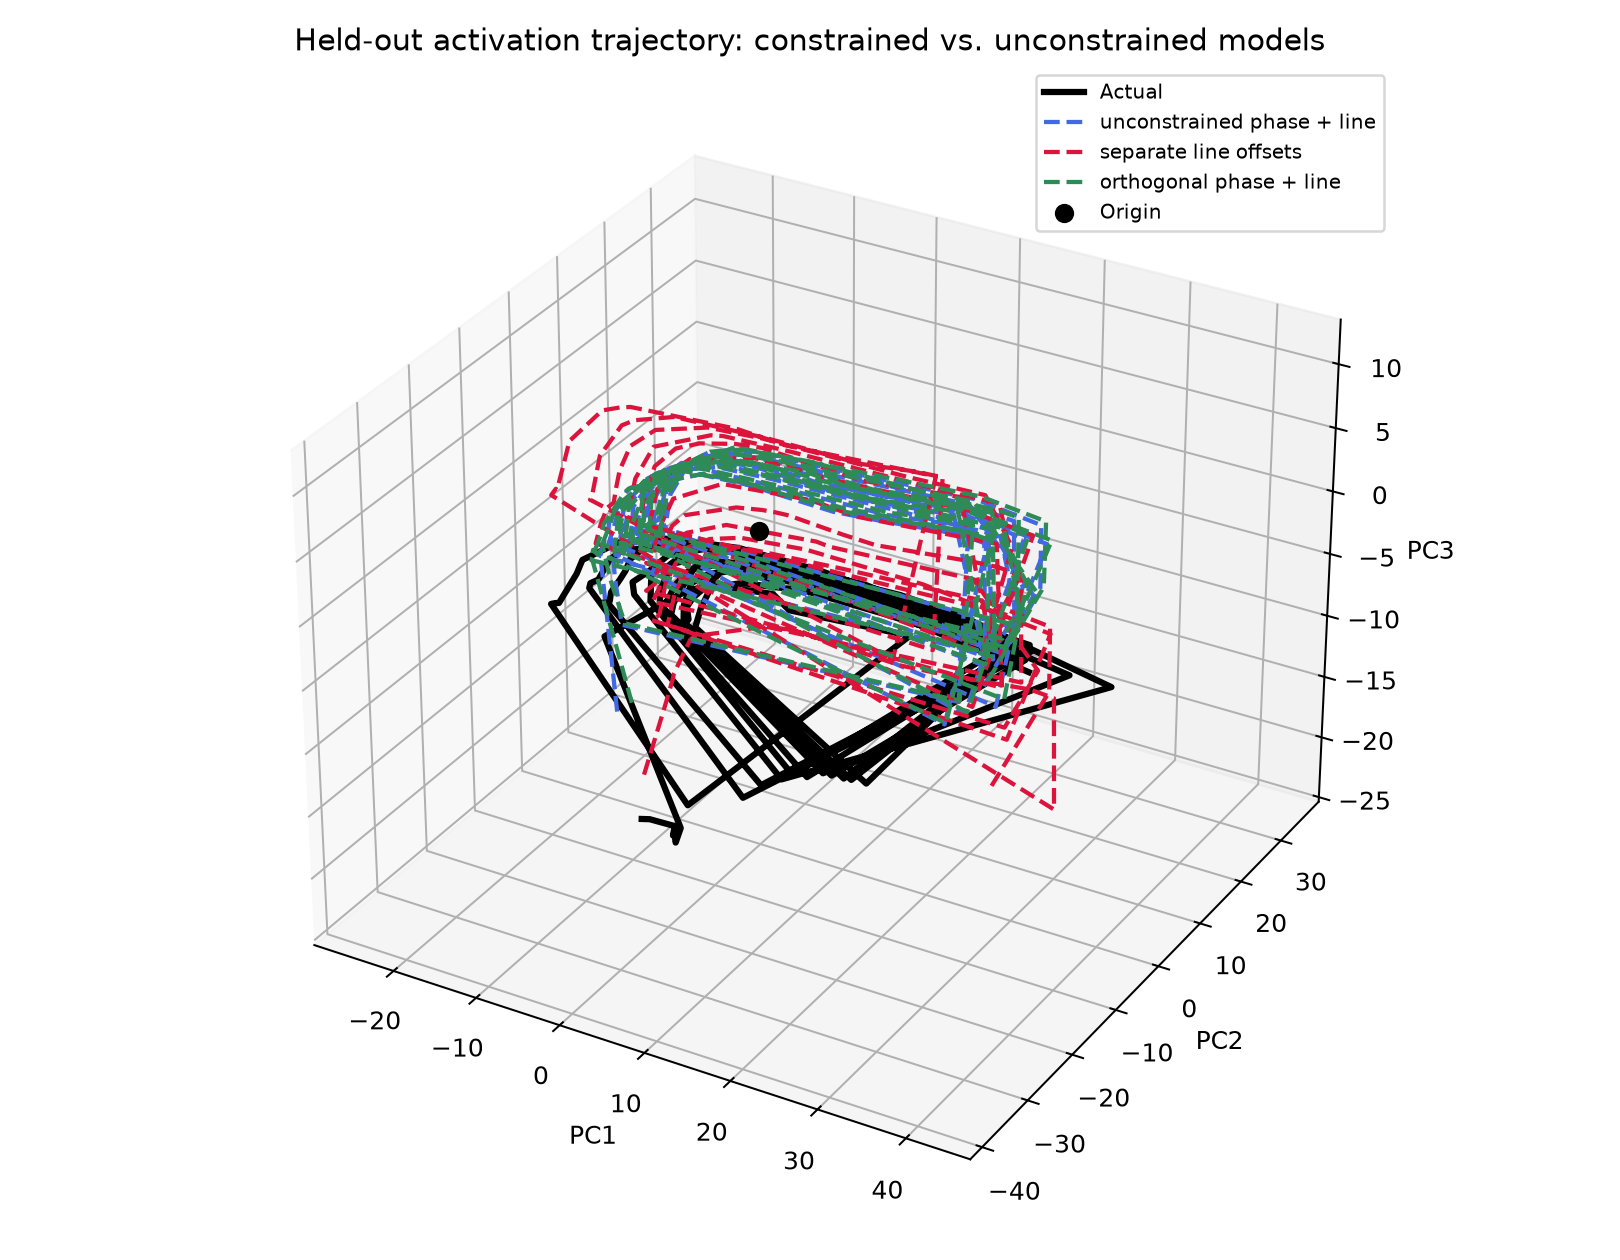
\includegraphics[width=\linewidth]{figures/constrained_line_phase_trajectory.png}
    \caption{Held-out activation trajectory before the final attention layer,
    shown in a global three-dimensional PCA basis. The actual trajectory is
    black; dashed curves show the unconstrained phase-plus-line model, the
    separate-line-offset model, and the orthogonally constrained model. The
    origin is shown in black.}
    \label{fig:constrained-line-phase}
\end{figure}

\begin{figure}[t]
    \centering
    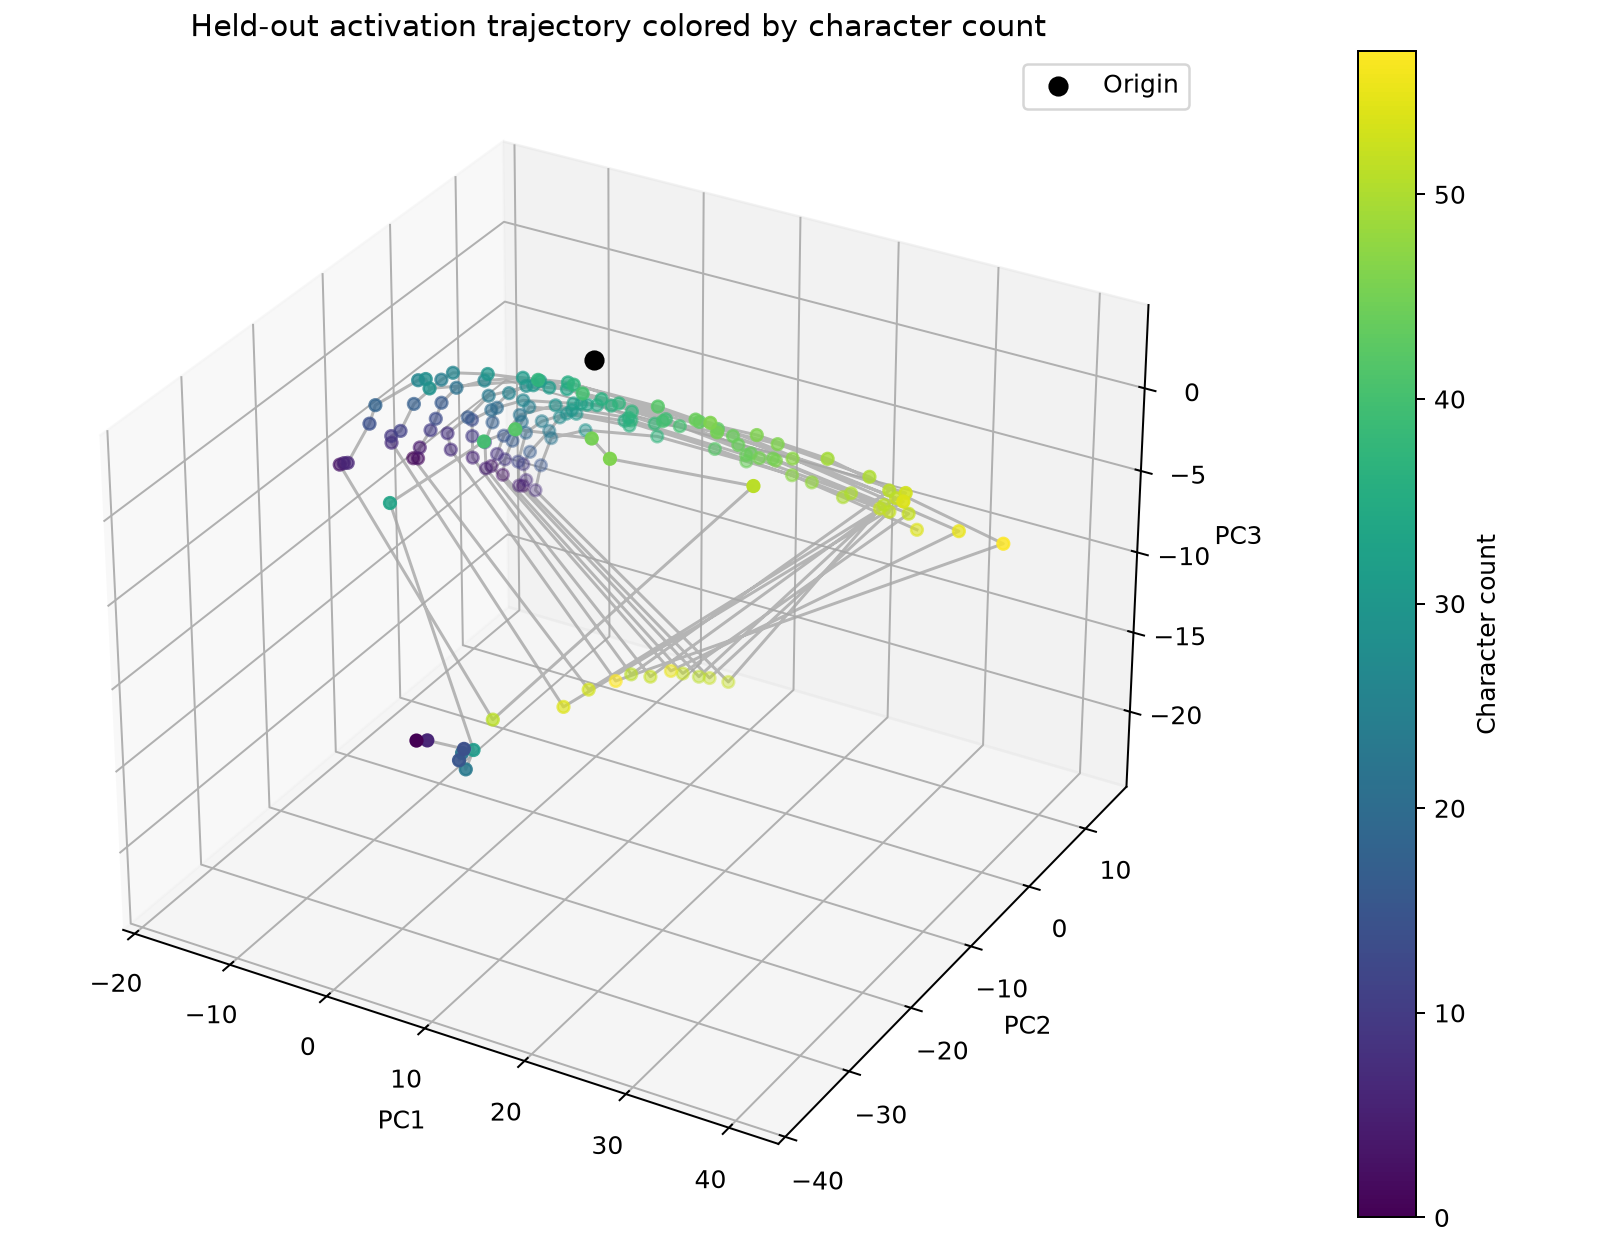
\includegraphics[width=\linewidth]{figures/activation_trajectory_character_count.png}
    \caption{A held-out trajectory in global PCA coordinates, with points
    colored by current character count.}
    \label{fig:activation-trajectory-count}
\end{figure}

\section{Current progress and next steps}

The codebase now contains a reproducible training and evaluation pipeline,
checkpointing, token-level tests, and a collection of interpretability
notebooks.  The existing analyses examine, among other things, attention to
previous newline tokens, probes for character counts, activation trajectories,
head ablations, and the geometry of query--key interactions near the final
prediction layer.  These experiments are intended to connect behavioral
success on line breaking to specific internal representations and circuits.

The next stage of the write-up will add quantitative training curves and a
clear account of the strongest mechanistic findings.  It will also be useful
to compare models trained with fixed versus variable line lengths, and to
separate the representation of the current line's character count from other
state variables such as line position or the identity of the previous newline.

\begin{thebibliography}{1}

\bibitem{gurnee2026manipulate}
Wes Gurnee, Emmanuel Ameisen, Isaac Kauvar, Julius Tarng, Adam Pearce,
Chris Olah, and Joshua Batson.
\newblock When Models Manipulate Manifolds: The Geometry of a Counting Task.
\newblock Anthropic, 2026.
\newblock \url{https://arxiv.org/abs/2601.04480}.

\end{thebibliography}

\end{document}
